%%%%%%%%%%%%%%%%%%%%%%%%%%%%%%%%%%%%%%%%%
% Beamer Presentation
% LaTeX Template
% Version 1.0 (10/11/12)
%
% This template has been downloaded from:
% http://www.LaTeXTemplates.com
%
% License:
% CC BY-NC-SA 3.0 (http://creativecommons.org/licenses/by-nc-sa/3.0/)
%
%%%%%%%%%%%%%%%%%%%%%%%%%%%%%%%%%%%%%%%%%

%----------------------------------------------------------------------------------------
%	PACKAGES AND THEMES
%----------------------------------------------------------------------------------------

\documentclass{beamer}

\mode<presentation> {

% The Beamer class comes with a number of default slide themes
% which change the colors and layouts of slides. Below this is a list
% of all the themes, uncomment each in turn to see what they look like.

%\usetheme{default}
%\usetheme{AnnArbor}
%\usetheme{Antibes}
%\usetheme{Bergen}
%\usetheme{Berkeley}
%\usetheme{Berlin}
%\usetheme{Boadilla}
%\usetheme{CambridgeUS}
%\usetheme{Copenhagen}
\usetheme{Darmstadt}
%\usetheme{Dresden}
%\usetheme{Frankfurt}
%\usetheme{Goettingen}
%\usetheme{Hannover}
%\usetheme{Ilmenau}
%\usetheme{JuanLesPins}
%\usetheme{Luebeck}
%\usetheme{Madrid}
%*\usetheme{Malmoe}
%\usetheme{Marburg}
%\usetheme{Montpellier}
%\usetheme{PaloAlto}
%\usetheme{Pittsburgh}
%\usetheme{Rochester}
%\usetheme{Singapore}
%\usetheme{Szeged}
%\usetheme{Warsaw}

% As well as themes, the Beamer class has a number of color themes
% for any slide theme. Uncomment each of these in turn to see how it
% changes the colors of your current slide theme.

%\usecolortheme{albatross}
%\usecolortheme{beaver}
%\usecolortheme{beetle}
%\usecolortheme{crane}
%\usecolortheme{dolphin}
%\usecolortheme{dove}
%\usecolortheme{fly}
%\usecolortheme{lily}
\usecolortheme{orchid}
%\usecolortheme{rose}
%\usecolortheme{seagull}
%\usecolortheme{seahorse}
%\usecolortheme{whale}
%\usecolortheme{wolverine}

%\setbeamertemplate{footline} % To remove the footer line in all slides uncomment this line
%\setbeamertemplate{footline}[page number] % To replace the footer line in all slides with a simple slide count uncomment this line

%\setbeamertemplate{navigation symbols}{} % To remove the navigation symbols from the bottom of all slides uncomment this line
}


\usepackage{graphicx} % Allows including images
\usepackage{booktabs} % Allows the use of \toprule, \midrule and \bottomrule in tables
\usepackage{xspace}
\usepackage{caption}
\usepackage{subfigure}
\usepackage[english,brazil]{babel}
\usepackage[utf8]{inputenc}

%Renomeia o nome padrao das figuras.
\renewcommand{\figurename}{Figura}
\renewcommand{\tablename}{Tabela}
%----------------------------------------------------------------------------------------
%	TITLE PAGE
%----------------------------------------------------------------------------------------

\title[Computação Gráfica]{Introdução à Computação Gráfica} % The short title appears at the bottom of every slide, the full title is only on the title page

\author{Uéliton Freitas} % Your name
\institute[UFMS] % Your institution as it will appear on the bottom of every slide, may be shorthand to save space
{
Universidade Católica Don Bosco - UCDB \\ % Your institution for the title page
\medskip
\textit{freitas.ueliton@gmail.com} % Your email address
}
\date{\today} % Date, can be changed to a custom date


\begin{document}

\begin{frame}
\titlepage % Print the title page as the first slide
\end{frame}

\begin{frame}
\frametitle{Sumário} % Table of contents slide, comment this block out to remove it
\tableofcontents % Throughout your presentation, if you choose to use \section{} and \subsection{} commands, these will automatically be printed on this slide as an overview of your presentation
\end{frame}




%----------------------------------------------------------------------------------------
%	PRESENTATION SLIDES
%----------------------------------------------------------------------------------------

%------------------------------------------------
\section{Introdução} 
%------------------------------------------------

%\section{Speeded-Up Robust Features - SURF} % A subsection can be created just before a set of slides with a common theme to further break down your presentation into chunks
%\section{Baf Of Features and Colors}

%\section{Refer\^encias}

%%%%%%%%%%%%%%%%%%%%%%%%%%%%%%%%%%%%%%%%%%%%%%%%%%%%%%%%%%%%%%%%%%%%%%%%%%%%%%%%%%%%%%%%%%
\begin{frame}
\frametitle{Introdução}

\begin{itemize}
	\item O que é Computação Gráfica?
	\begin{figure}[htb!]
  		\centering
    			\subfigure[Dota 2]{%
      		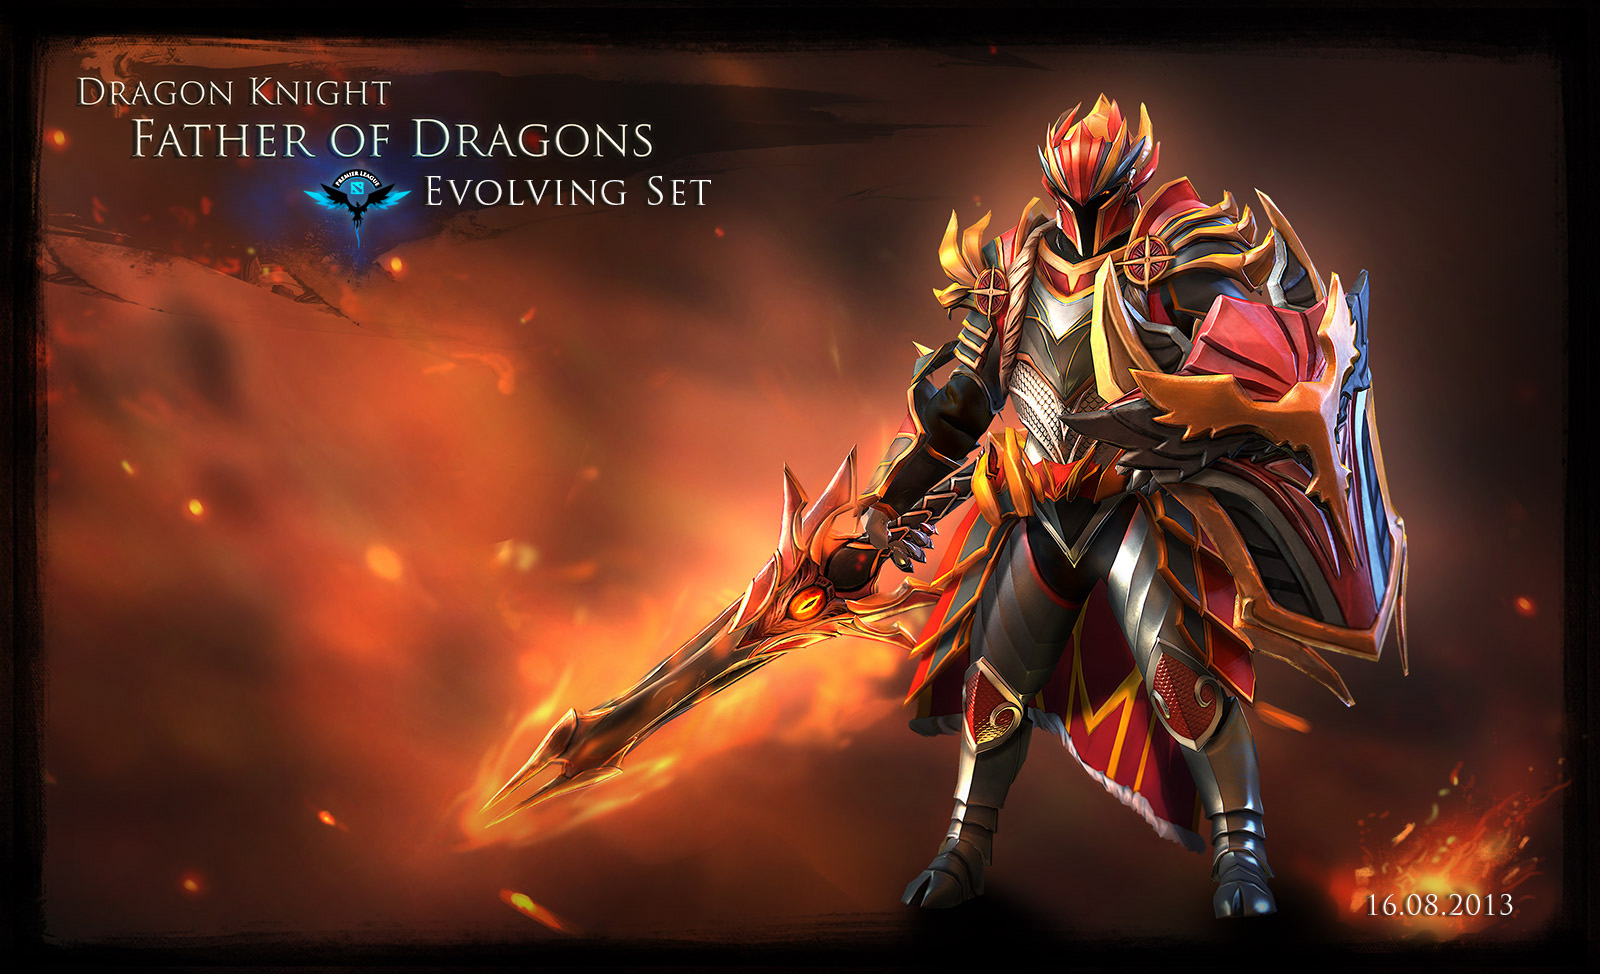
\includegraphics[width=0.3\textwidth]{Figures/dk}}\qquad
   			\subfigure[Battle Field 4]{%
     		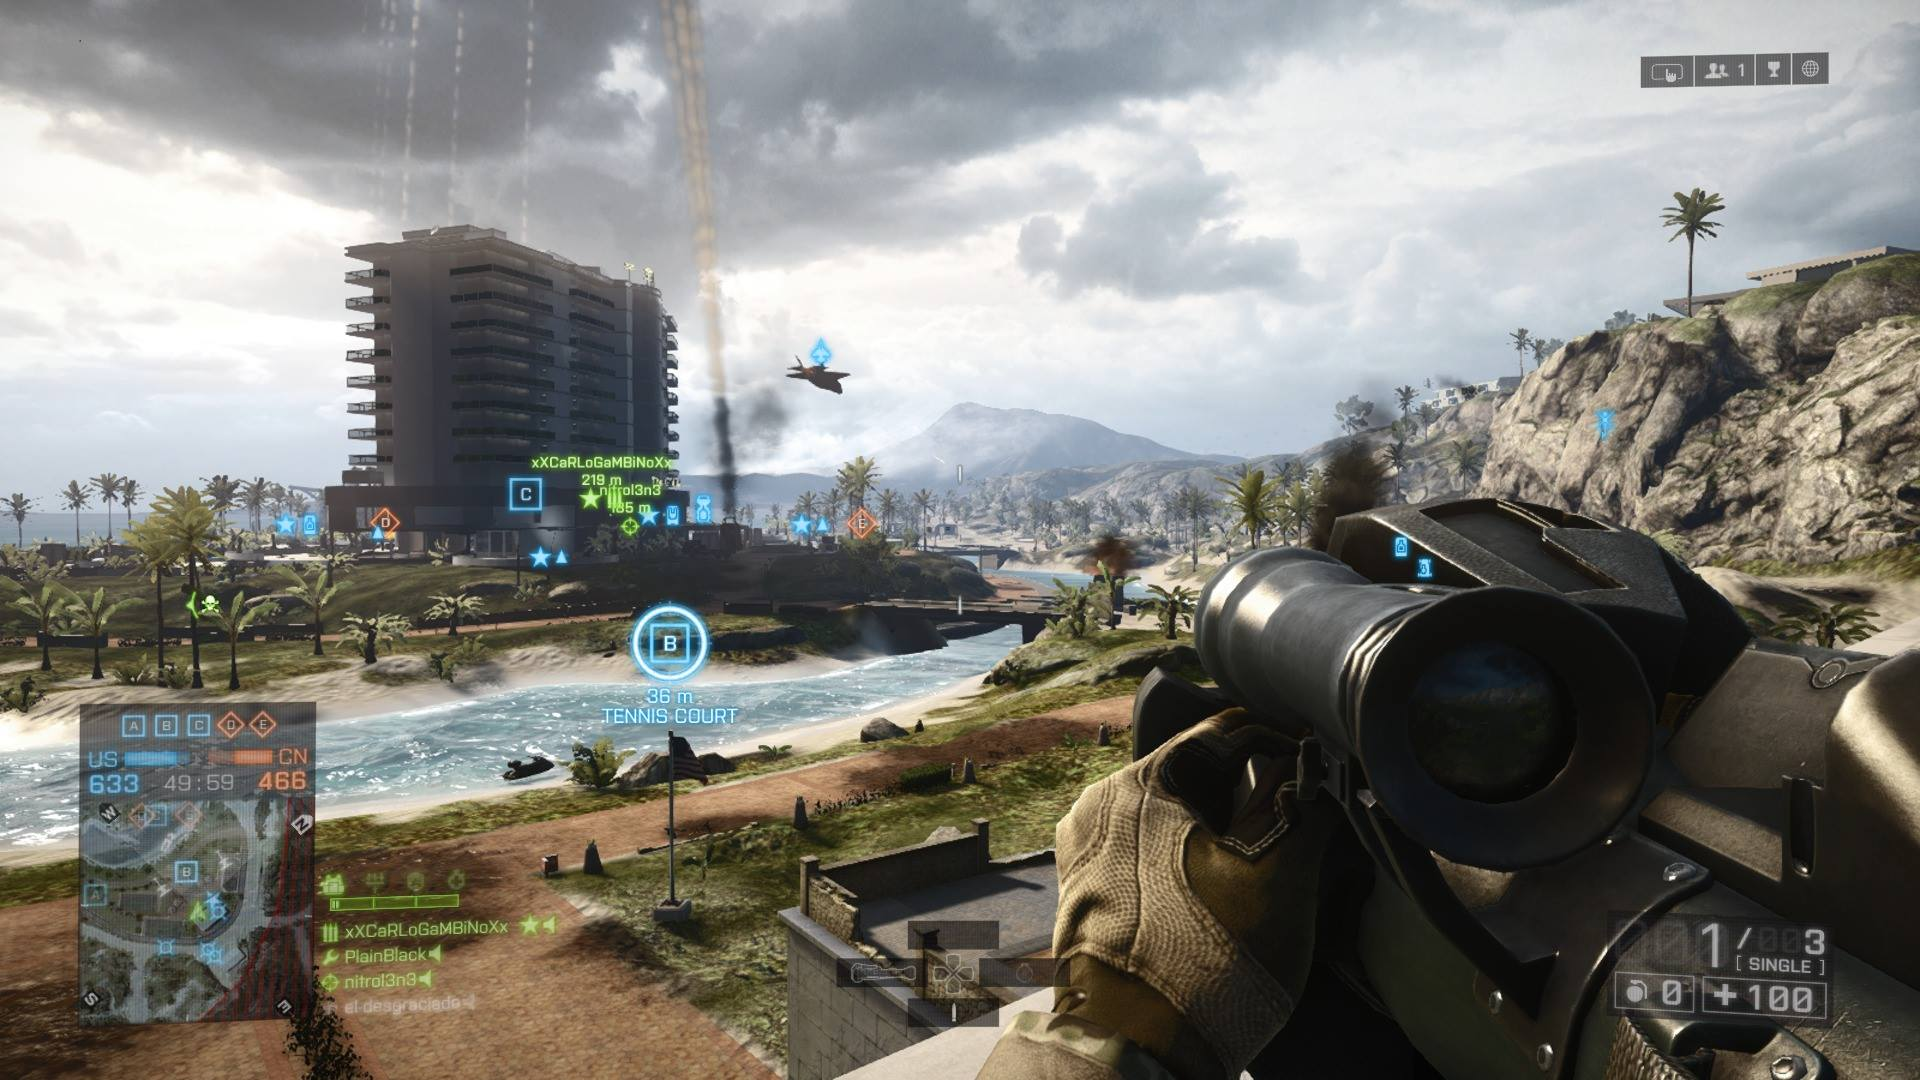
\includegraphics[width=0.3\textwidth]{Figures/bf4}}\qquad
     		\subfigure[Como Treinar seu Dragão 2]{%
     		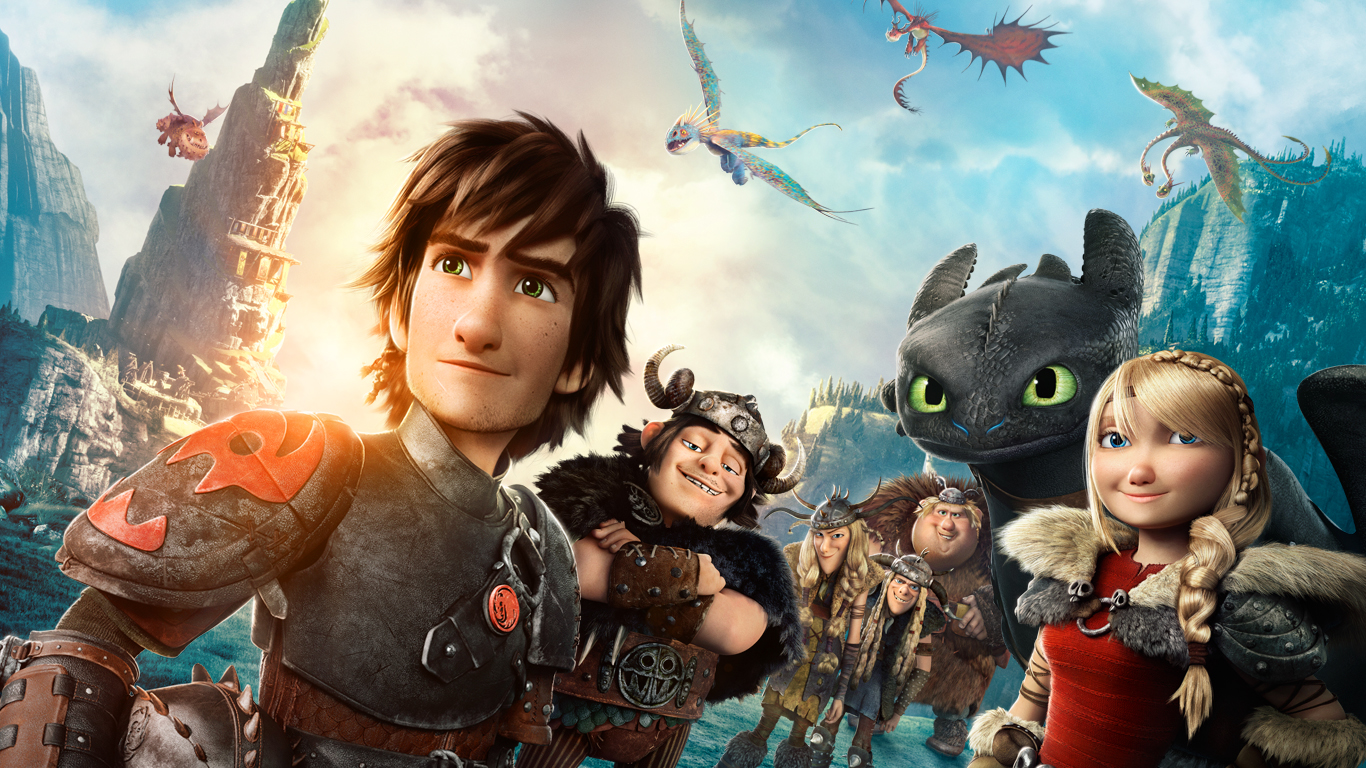
\includegraphics[width=0.3\textwidth]{Figures/htd}}\qquad
     		\subfigure[Projeto de um Avião]{%
     		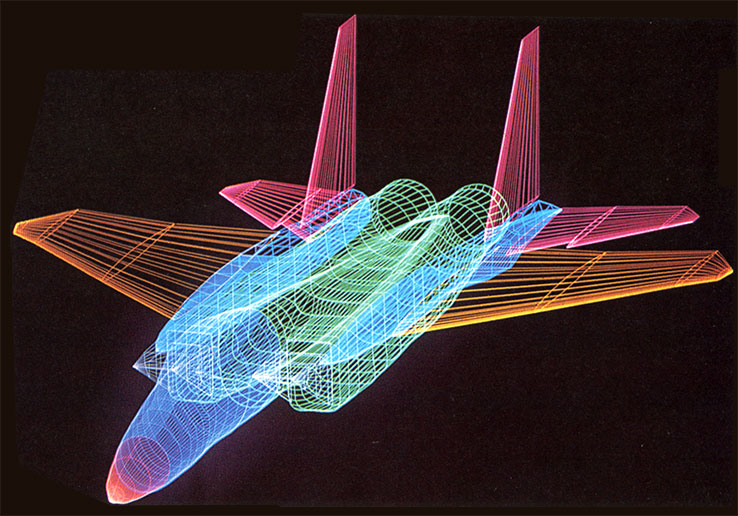
\includegraphics[width=0.3\textwidth]{Figures/plane}}\qquad
  		\label{iep}
	\end{figure}

\end{itemize}

	
\end{frame}

%%%%%%%%%%%%%%%%%%%%%%%%%%%%%%%%%%%%%%%%%%%%%%%%%%%%%%%%%%%%%%%%%%%%%%%%%%%%%%%%%%%%%%%%%%

\begin{frame}
\frametitle{Introdução}

\begin{itemize}
	\item O que é Computação Gráfica? \\
	\textbf{Computação Gráfica} é a ciência e arte da comunicação visual via display de um computador e integração dos dispositivos envolvidos.
	\begin{figure}[htb!]
  \centering
    \subfigure[Periféricos utilizados em Computação gráfica.]{\label{dota}%
      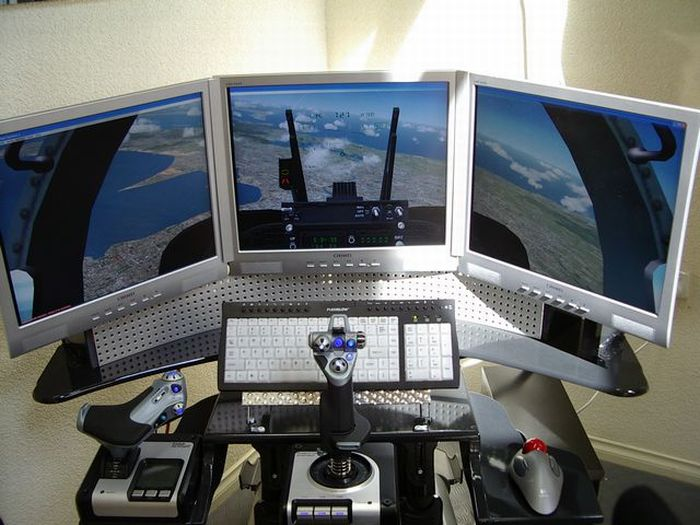
\includegraphics[width=0.3\textwidth]{Figures/pc}}\qquad
   \subfigure[Simulador de Voo da NASA.]{\label{bf4}%
     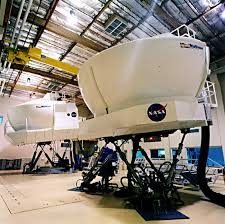
\includegraphics[width=0.3\textwidth]{Figures/nasa}}\qquad
  \label{iep}
\end{figure}

\end{itemize}
\end{frame}

%%%%%%%%%%%%%%%%%%%%%%%%%%%%%%%%%%%%%%%%%%%%%%%%%%%%%%%%%%%%%%%%%%%%%%%%%%%%%%%%%%%%%%%%%%

\begin{frame}
\frametitle{Introdução}

	
	\begin{block}{O que é Computação Gráfica?}
		\begin{itemize}
			\item<1-> \textbf{Computação Gráfica} é a ciência e arte da comunicação visual via display de um computador e integração dos dispositivos envolvidos.
		\end{itemize}
	\end{block}

	\begin{block}{O que a Computação Gráfica Aborda?}
		\begin{itemize}
			\item<2-> Técnicas para geração, exibição e manipulação e interpretação de modelos de imagens utilizando o computador.
		\end{itemize}
	\end{block}
	
	\begin{block}{Tipos de Usuários}
		\begin{itemize}
				\item<3-> Ciência, engenharia, medicina, arte, publicidade, ...
		\end{itemize}
	\end{block}	
	
	\begin{block}{Maiores Informações Sobre a Área} 
		\begin{itemize}
				\item<4-> ACM SIGGRAPH (http://www.siggraph.org/)
		\end{itemize}
	\end{block}
	
	
\end{frame}

%%%%%%%%%%%%%%%%%%%%%%%%%%%%%%%%%%%%%%%%%%%%%%%%%%%%%%%%%%%%%%%%%%%%%%%%%%%%%%%%%%%%%%%%%%


\section{Evolução da Computação Gráfica}
\subsection{História}
\begin{frame}
\frametitle{Evolução da Computação Gráfica}

\begin{block}{Sketchpad - 1963}
	\begin{itemize}
		\item<1-> Ivan Sutherland apresenta um sistema de que desenvolvia em seu Ph.D no MIT.
		\item<1-> Programa de manipulação e criação de elementos 2D em um monitor de vídeo.
		\item<1-> Utilizava uma \textbf{caneta óptica} como dispositivo de entrada e o monitor como dispositivo de saída.
		
		\item<1-> Primeira tentativa de usar dispositivo de vídeo como dispositivo de integração assim como o computador para gerar e exibir figuras.
	\end{itemize}
	
\end{block}

\end{frame}

%%%%%%%%%%%%%%%%%%%%%%%%%%%%%%%%%%%%%%%%%%%%%%%%%%%%%%%%%%%%%%%%%%%%%%%%%%%%%%%%%%%%%%%%%%


\begin{frame}
\frametitle{Evolução da Computação Gráfica}
	\begin{figure}[!h]
			\begin{center}
			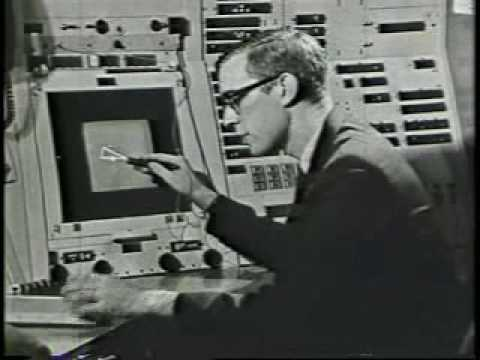
\includegraphics[width=0.5\textwidth]{Figures/ivan}
			\caption{Ivan Sutherland no console TX-2.}\label{ivan}
			\end{center}
	\end{figure}
\end{frame}

%%%%%%%%%%%%%%%%%%%%%%%%%%%%%%%%%%%%%%%%%%%%%%%%%%%%%%%%%%%%%%%%%%%%%%%%%%%%%%%%%%%%%%%%%%


\begin{frame}
\frametitle{Evolução da Computação Gráfica}

\begin{block}{História}

	\begin{itemize}
		\item<1-> Dispositivos de Exibição:
		\begin{itemize}
			\item<1-> Natureza analógica:vector graphics.
			\item<1-> Os desenhos eram formados por segmentos de retas.
			\item<1-> Tecnologia cara e sem cores.
		\end{itemize}
		\item<1-> Primeiros programas CAD  (Computer Aided Design).
		\item<1-> Pouca iteração com o usuário e a tecnologia como um todo era muito cara.
	
	\end{itemize}
\end{block}

\end{frame}

%%%%%%%%%%%%%%%%%%%%%%%%%%%%%%%%%%%%%%%%%%%%%%%%%%%%%%%%%%%%%%%%%%%%%%%%%%%%%%%%%%%%%%%%%%


\begin{frame}
\frametitle{Evolução da Computação Gráfica}

	\begin{figure}[!h]
		\begin{center}
			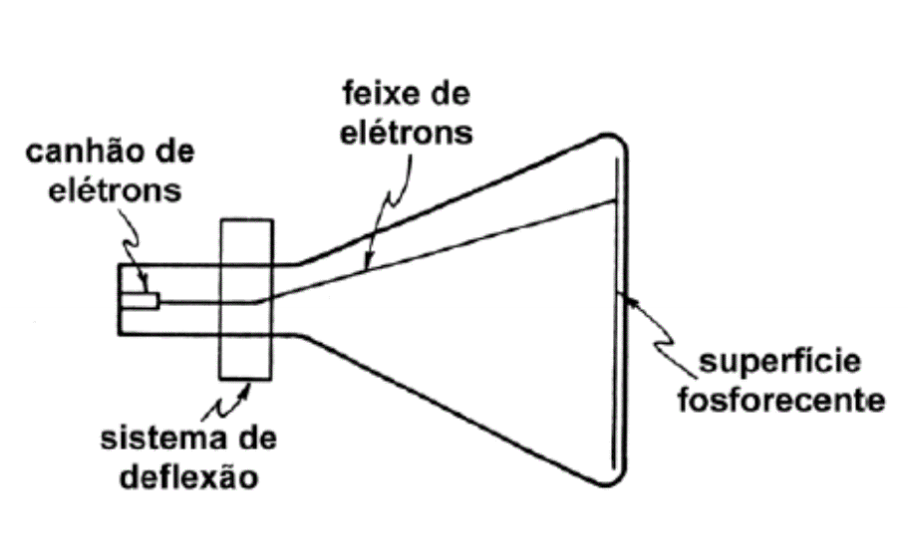
\includegraphics[width=0.9\textwidth]{Figures/crt}
			\caption{CRT.}
		\end{center}
		
	\end{figure}

\end{frame}

%%%%%%%%%%%%%%%%%%%%%%%%%%%%%%%%%%%%%%%%%%%%%%%%%%%%%%%%%%%%%%%%%%%%%%%%%%%%%%%%%%%%%%%%%%


\begin{frame}
\frametitle{Evolução da Computação Gráfica}

\begin{block}{Década de 70}
		\begin{itemize}
			\item<1-> Disseminação de aplicativos.
			\item<1-> Evolução da Computação Gráfica de \textit{hardware}.
				\begin{itemize}
					\item Surgimento da \textbf{tecnologia matricial} (\textit{raster graphics}).
					\item Imagens formadas por matrizes de pontos ou \textit{pixels}.
					\item Tecnologia mais \textbf{barata}.
					\item Possibilita o uso de cores e preenchimento das figuras.
					\item \textbf{Aliasing}.
				\end{itemize}
			\item Aumento da capacidade gráfica.
			\item Melhores dispositivos de integração (Mouse 1968).
			\item Novos paradigmas em IHC (criação de janelas).
		\end{itemize}
\end{block}

\end{frame}


%%%%%%%%%%%%%%%%%%%%%%%%%%%%%%%%%%%%%%%%%%%%%%%%%%%%%%%%%%%%%%%%%%%%%%%%%%%%%%%%%%%%%%%%%%


\begin{frame}
\frametitle{Evolução da Computação Gráfica}

	\begin{figure}[!h]
		\begin{center}
			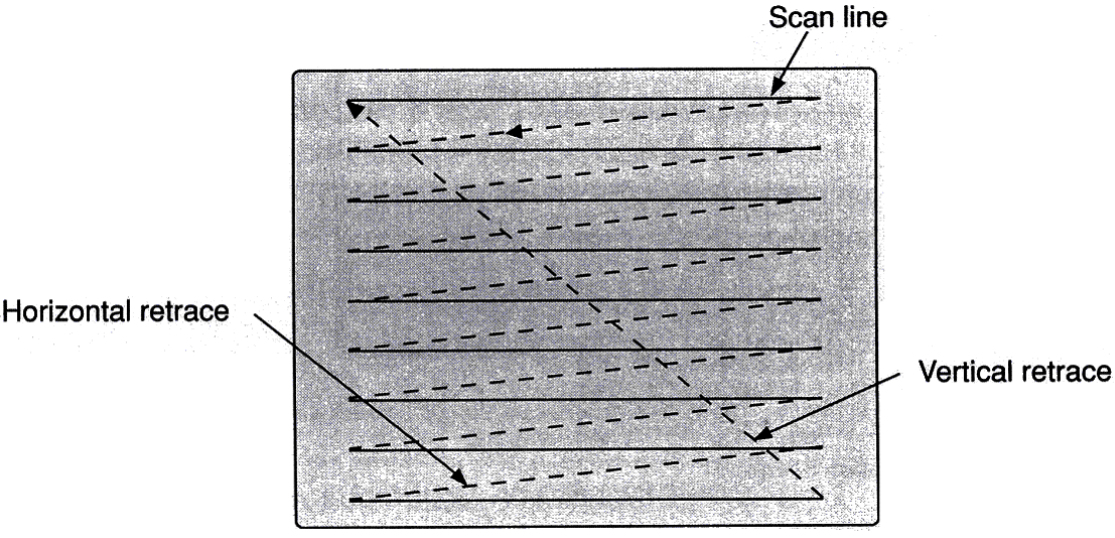
\includegraphics[width=0.9\textwidth]{Figures/matrixcrt}
			\caption{CRT Matricial.}
		\end{center}
		
	\end{figure}

\end{frame}

%%%%%%%%%%%%%%%%%%%%%%%%%%%%%%%%%%%%%%%%%%%%%%%%%%%%%%%%%%%%%%%%%%%%%%%%%%%%%%%%%%%%%%%%%%


\begin{frame}
\frametitle{Evolução da Computação Gráfica}

\begin{block} {Pixel}
	O \textbf{Pixel} é uma pequena área da imagem armazenada no \textbf{Frame Buffer}.
	
\end{block}

	\begin{figure}[!h]
		\begin{center}
			\subfigure[Imagem original.]{
      			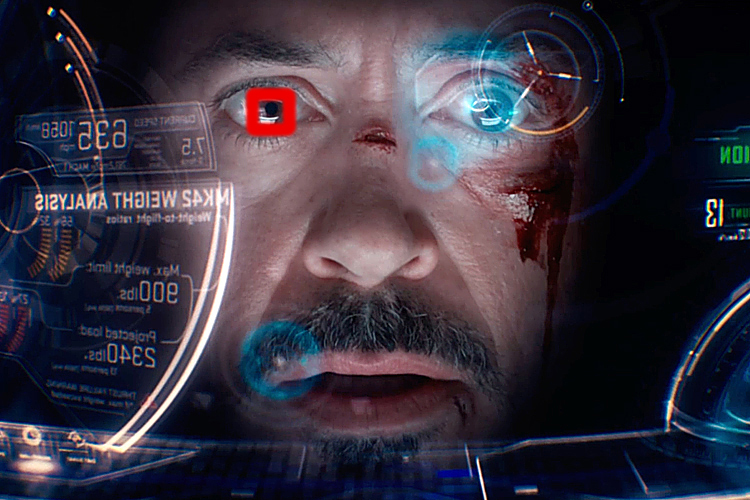
\includegraphics[width=0.6\textwidth]{Figures/ironman}}\qquad
      		\subfigure[Imagen aumentada.]{
      			
\includegraphics[width=0.3\textwidth]{Figures/tumb}}\qquad
		\end{center}
		
	\end{figure}

\end{frame}

%%%%%%%%%%%%%%%%%%%%%%%%%%%%%%%%%%%%%%%%%%%%%%%%%%%%%%%%%%%%%%%%%%%%%%%%%%%%%%%%%%%%%%%%%%


\begin{frame}
\frametitle{Evolução da Computação Gráfica}

\begin{block} {Pixel}
	O \textbf{Pixel} é uma pequena área da imagem armazenada no \textbf{Frame Buffer}.
	
\end{block}

	\begin{figure}[!h]
		\begin{center}
			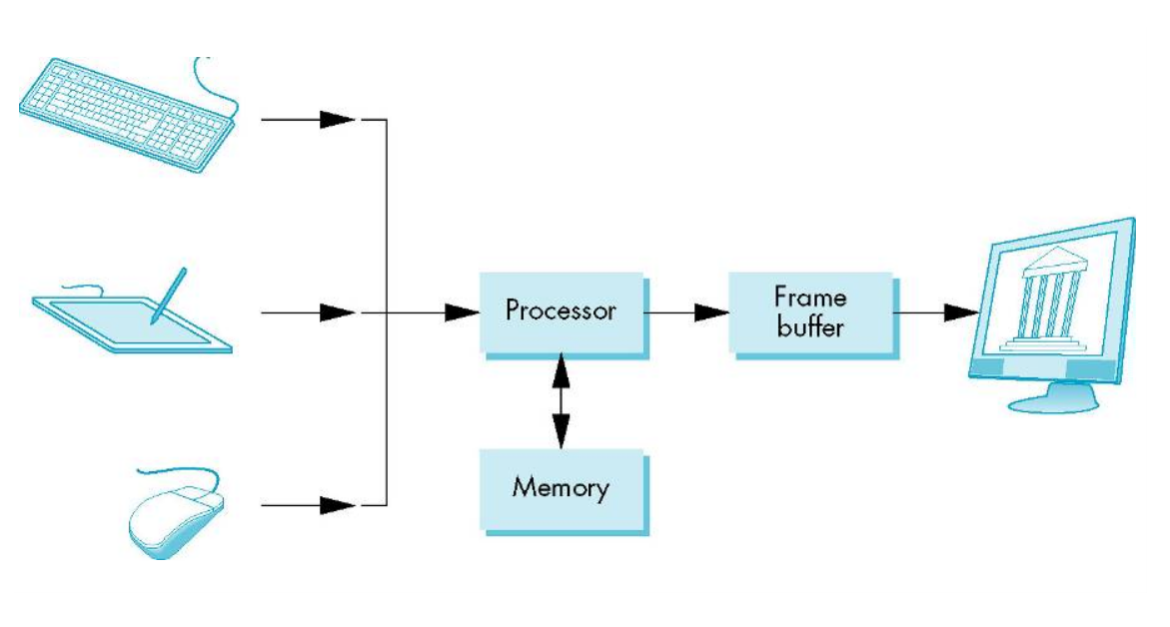
\includegraphics[width=0.8\textwidth]{Figures/framebuffer}
			\caption{Representação do Frame Buffer.}
		\end{center}
		
	\end{figure}

\end{frame}

%%%%%%%%%%%%%%%%%%%%%%%%%%%%%%%%%%%%%%%%%%%%%%%%%%%%%%%%%%%%%%%%%%%%%%%%%%%%%%%%%%%%%%%%%%


\begin{frame}
\frametitle{Evolução da Computação Gráfica}

\begin{block}{Década de 80}
		\begin{itemize}
			\item<1-> Pacotes Gráficos.
				\begin{itemize}
					\item \textbf{Portabilidade} (Independência de dispositivos).
					\item Reutilização.
					\item API's: OpenGL. Aplicativos independentes de SO (sistemas de janelas etc.).
				\end{itemize}
			\item \textbf{Computação Gráfica 3D}
				\begin{itemize}
					\item Representação dos objetos no espaço 3D.
				\end{itemize}
			
		\end{itemize}
\end{block}

\end{frame}


%%%%%%%%%%%%%%%%%%%%%%%%%%%%%%%%%%%%%%%%%%%%%%%%%%%%%%%%%%%%%%%%%%%%%%%%%%%%%%%%%%%%%%%%%%


\begin{frame}
\frametitle{Evolução da Computação Gráfica}

	\begin{figure}[!h]
		\begin{center}
			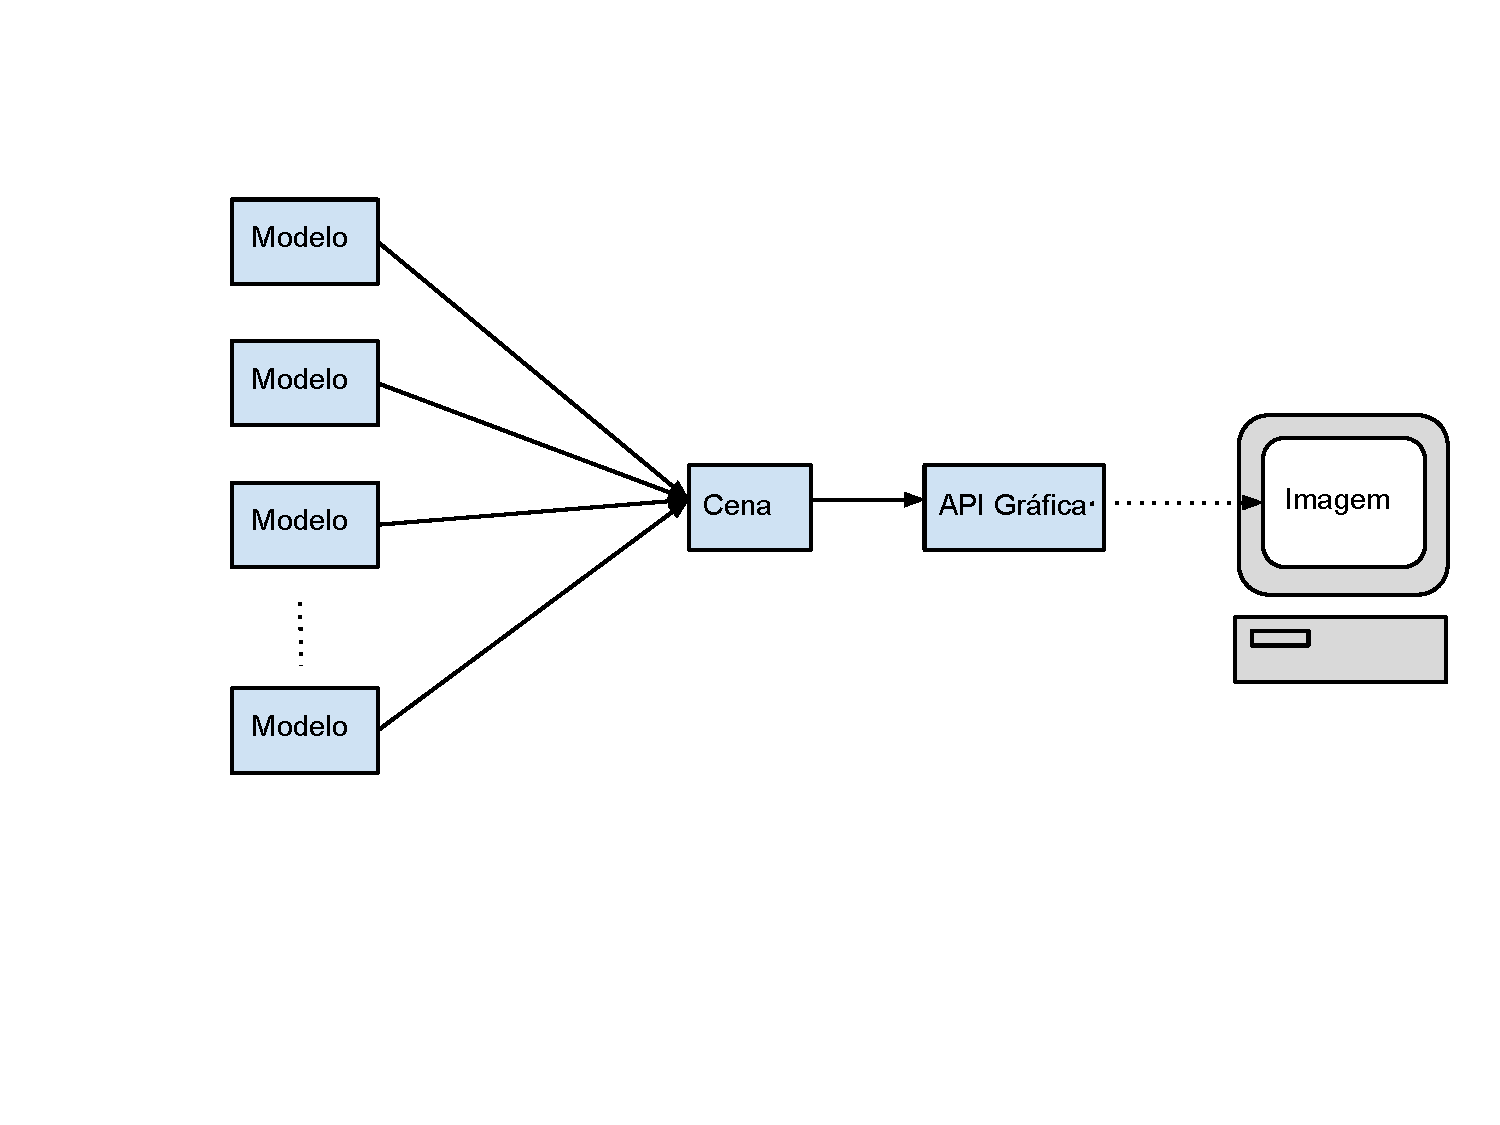
\includegraphics[width=0.8\textwidth]{Figures/ModelagemCG}
			\caption{Sistema Gráfico.}
		\end{center}
		
	\end{figure}

\end{frame}

%%%%%%%%%%%%%%%%%%%%%%%%%%%%%%%%%%%%%%%%%%%%%%%%%%%%%%%%%%%%%%%%%%%%%%%%%%%%%%%%%%%%%%%%%%


\begin{frame}
\frametitle{Evolução da Computação Gráfica}

\begin{block}{Outras Inovações}

	\begin{itemize}
		\item<1-> Técnicas de criação de mundo 3D:
		\begin{itemize}
			\item \textbf{Modelagem} - Criação da representação de um objeto.
				\begin{itemize}
					\item Informações geométricas.
					\item Informações sobre as fontes de luz e observador.
					\item Informações sobre os materiais do objeto.
					\item Poligonização: Aproximação de uma forma de um objeto por meio de uma malha de faces poligonais (como triângulos). 
				\end{itemize}
			\item \textbf{Renderização} e Animação - Meios de se exibir o objeto 
				\begin{itemize}
					\item Geração de uma imagem a partir dos modelos.
					\item Simulações da iteração de fontes de luz.
				\end{itemize}
			
		\end{itemize}
	\end{itemize}
\end{block}

\end{frame}


%%%%%%%%%%%%%%%%%%%%%%%%%%%%%%%%%%%%%%%%%%%%%%%%%%%%%%%%%%%%%%%%%%%%%%%%%%%%%%%%%%%%%%%%%%


\begin{frame}
\frametitle{Evolução da Computação Gráfica}

\begin{block}{Década de 90}
		\begin{itemize}
			\item Gama de técnicas em síntese de imagens.
				\begin{itemize}
					\item Estratégias clássicas de modelagem: fronteiras, CSG, octrees...
					\item Estratégias para descrições de modelos: varreduras, formulações matemáticas para definições alternativas para curvas e superfícies.
					\item Estratégias alternativas de modelagens: fractais, partículas..
					\item Estratégias de rendering sofisticadas: ray tracing, mapeamento de textura. 
				\end{itemize}
			\item As áreas relacionadas amadureceram.
			
		\end{itemize}
\end{block}

\end{frame}


%%%%%%%%%%%%%%%%%%%%%%%%%%%%%%%%%%%%%%%%%%%%%%%%%%%%%%%%%%%%%%%%%%%%%%%%%%%%%%%%%%%%%%%%%%

\section{Hardware}
\begin{frame}
\frametitle{Hardware}

	\begin{figure}[!h]
		\begin{center}
			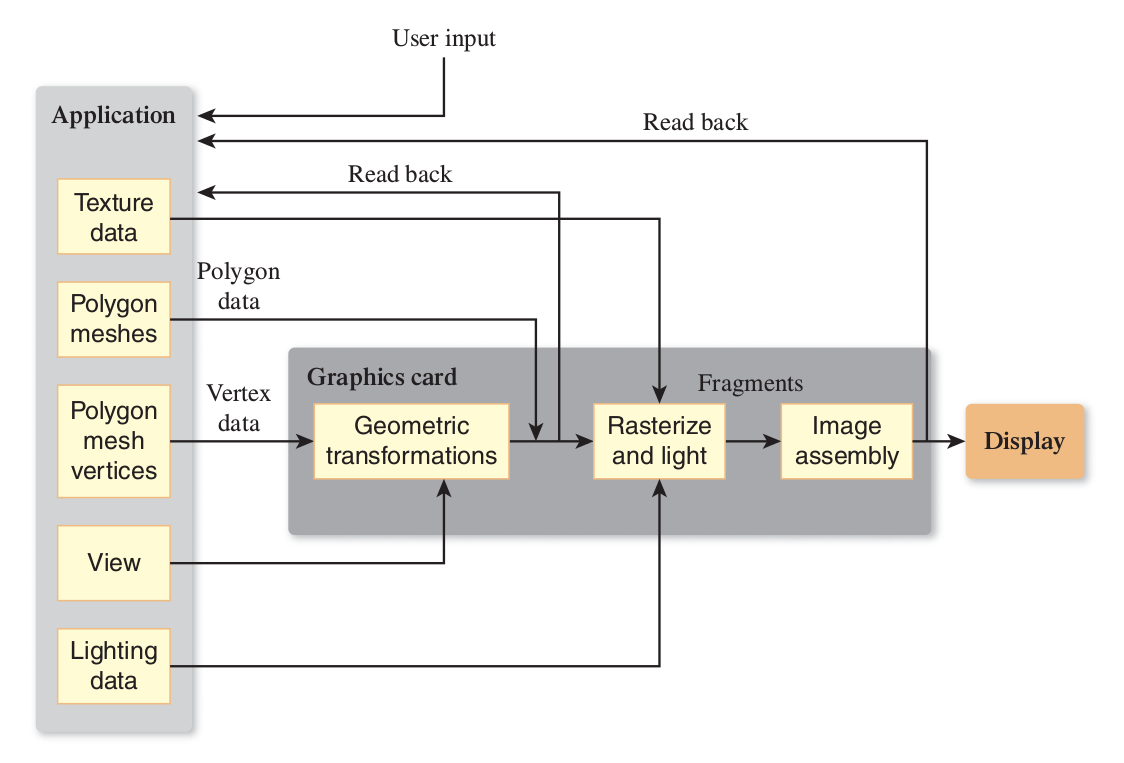
\includegraphics[width=0.8\textwidth]{Figures/graphicPipeline}
			\caption{Pipeline Gráfico.}
		\end{center}
		
	\end{figure}

\end{frame}


%%%%%%%%%%%%%%%%%%%%%%%%%%%%%%%%%%%%%%%%%%%%%%%%%%%%%%%%%%%%%%%%%%%%%%%%%%%%%%%%%%%%%%%%%%

\subsection{Dispositivos de Exibição}
\begin{frame}
\frametitle{Dispositivos de Exibição}
	
	\begin{block}{Dispositivos de Exibição de Natureza Analógica}
		\begin{itemize}
			\item Gráficos vetoriais.
			\item Imagens formadas a partir de segmentos de retas.
			\item Gerados por meio dos ``\textit{Display Files}''.
		\end{itemize}
	\end{block}
	
	\begin{block}{Dispositivos de Exibição de Natureza Digital}
		\begin{itemize}
			\item Gráficos Matriciais.
			\item Imagens formadas a partir do preenchimento de matrizes de pixels.
			\item Geradas a partir do \textit{Frame Buffer}.
		\end{itemize}
	\end{block}

\end{frame}

%%%%%%%%%%%%%%%%%%%%%%%%%%%%%%%%%%%%%%%%%%%%%%%%%%%%%%%%%%%%%%%%%%%%%%%%%%%%%%%%%%%%%%%%%%
\subsubsection{Dispositivo de Exibição Vetorial}
\begin{frame}
\frametitle{Dispositivo de Exibição Vetorial}

	\begin{figure}[!h]
		\begin{center}
			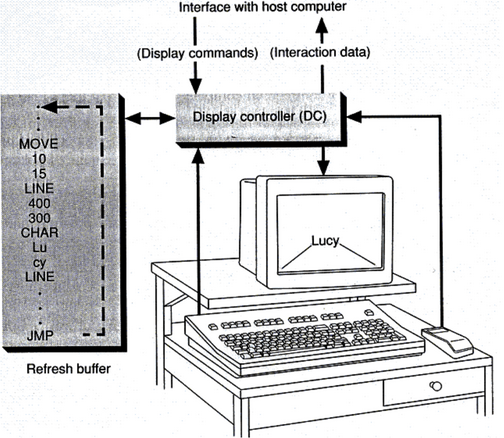
\includegraphics[width=0.8\textwidth]{Figures/vecDisp}
		\end{center}
		
	\end{figure}

\end{frame}

%%%%%%%%%%%%%%%%%%%%%%%%%%%%%%%%%%%%%%%%%%%%%%%%%%%%%%%%%%%%%%%%%%%%%%%%%%%%%%%%%%%%%%%%%%

\begin{frame}
\frametitle{Dispositivos Vetoriais}
	
	\begin{block}{Geração de Imagens Vetoriais }
		\begin{itemize}
			\item As cenas das imagens são mantidas nos ``\textit{Display Files}''.
			\item O interpretador de vídeo interpreta os dados contidos nos``\textit{Display Files}'' .
			\item Há vários comandos como:
				\begin{itemize}
					\item Posiciona ponto (x,y).
					\item Traçar linha do ponto atual até o ponto (x,y).
				\end{itemize}
		\end{itemize}
	\end{block}

\end{frame}

%%%%%%%%%%%%%%%%%%%%%%%%%%%%%%%%%%%%%%%%%%%%%%%%%%%%%%%%%%%%%%%%%%%%%%%%%%%%%%%%%%%%%%%%%%

\begin{frame}
\frametitle{Dispositivos Vetoriais}
	
	\begin{block}{Características dos Dispositivos Vetoriais}
		\begin{itemize}
			\item Representação, manipulação e visualização da sena são representadas por formas geométricas dos objetos.
			\item A restauração da tela é feita retraçando os vetores que definem os objetos.
		\end{itemize}
	\end{block}

\end{frame}

%%%%%%%%%%%%%%%%%%%%%%%%%%%%%%%%%%%%%%%%%%%%%%%%%%%%%%%%%%%%%%%%%%%%%%%%%%%%%%%%%%%%%%%%%%

\begin{frame}
\frametitle{Dispositivos Vetoriais}
	
	\begin{block}{Vantagens dos Dispositivos Vetoriais}
		\begin{itemize}
			\item As operações podem ser aplicadas diretamente nos objetos.
			\item Transformações podem ser aplicadas apenas aos pontos externos.
			\item Pouca memória para cenas complexas.
			\item Não contém cerrilhamento (\textit{Aliasing}).
		\end{itemize}
	\end{block}

\end{frame}

%%%%%%%%%%%%%%%%%%%%%%%%%%%%%%%%%%%%%%%%%%%%%%%%%%%%%%%%%%%%%%%%%%%%%%%%%%%%%%%%%%%%%%%%%%

\begin{frame}
\frametitle{Dispositivos Vetoriais}
	
	\begin{block}{Desvantagens dos Dispositivos Vetoriais}
		\begin{itemize}
			\item Difícil preencher o interior dos objetos.
			\item \textit{Fliker} (a imagem fica ``Piscando'') nas imagens.
			\item A restauração da tela depende da complexidade da cena.
			\item Alto custo.
			\item Tecnologia ultrapassada.
		\end{itemize}
	\end{block}

\end{frame}


%%%%%%%%%%%%%%%%%%%%%%%%%%%%%%%%%%%%%%%%%%%%%%%%%%%%%%%%%%%%%%%%%%%%%%%%%%%%%%%%%%%%%%%%%%
\subsubsection{Dispositivo de Exibição Matricial}
\begin{frame}
\frametitle{Dispositivo de Exibição Matricial}

	\begin{figure}[!h]
		\begin{center}
			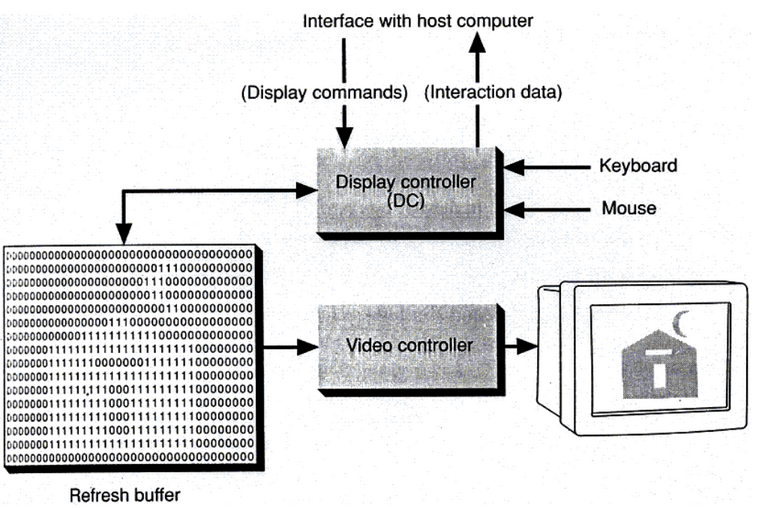
\includegraphics[width=0.8\textwidth]{Figures/matrixDisp}
		\end{center}
		
	\end{figure}

\end{frame}


%%%%%%%%%%%%%%%%%%%%%%%%%%%%%%%%%%%%%%%%%%%%%%%%%%%%%%%%%%%%%%%%%%%%%%%%%%%%%%%%%%%%%%%%%%

\begin{frame}
\frametitle{Dispositivo de Exibição Matricial}

	\begin{figure}[!h]
		\begin{center}
			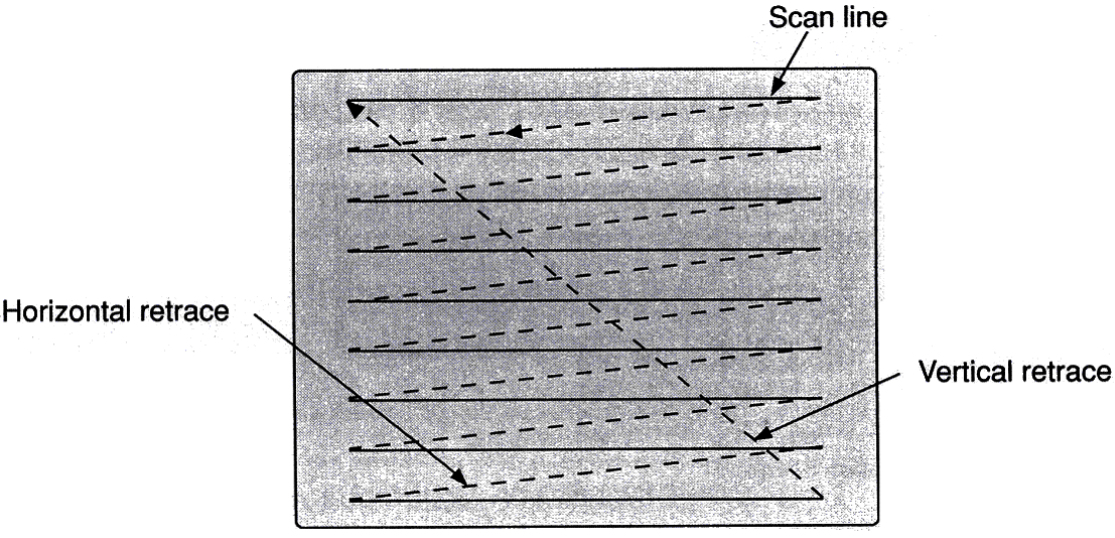
\includegraphics[width=0.8\textwidth]{Figures/matrixcrt}
		\end{center}
	\end{figure}
	
	\begin{block}{Modo de Atualização de Tela}
		\begin{itemize}
			\item Não entrelaçado: linha por linha (50-80 Hz).
			\item Entrelaçado: linhas pares e ímpares (60 Hz).
		\end{itemize}
	\end{block}

\end{frame}


%%%%%%%%%%%%%%%%%%%%%%%%%%%%%%%%%%%%%%%%%%%%%%%%%%%%%%%%%%%%%%%%%%%%%%%%%%%%%%%%%%%%%%%%%%

\begin{frame}
\frametitle{Dispositivo de Exibição Matricial}
	
	\begin{block}{Geração de Imagens Matriciais}
		\begin{itemize}
			\item As cenas são armazenadas no \textit{Frame Buffer}, que contém uma posição associada a cada pixel.
			\item Para cada pixel há um valor associado que contém a intensidade e a cor com que mesmo será traçado.
			\item Todos os objetos são pixels.
		\end{itemize}
	\end{block}

\end{frame}


%%%%%%%%%%%%%%%%%%%%%%%%%%%%%%%%%%%%%%%%%%%%%%%%%%%%%%%%%%%%%%%%%%%%%%%%%%%%%%%%%%%%%%%%%%

\begin{frame}
\frametitle{Dispositivo de Exibição Matricial}

	\begin{figure}[!h]
		\begin{center}
			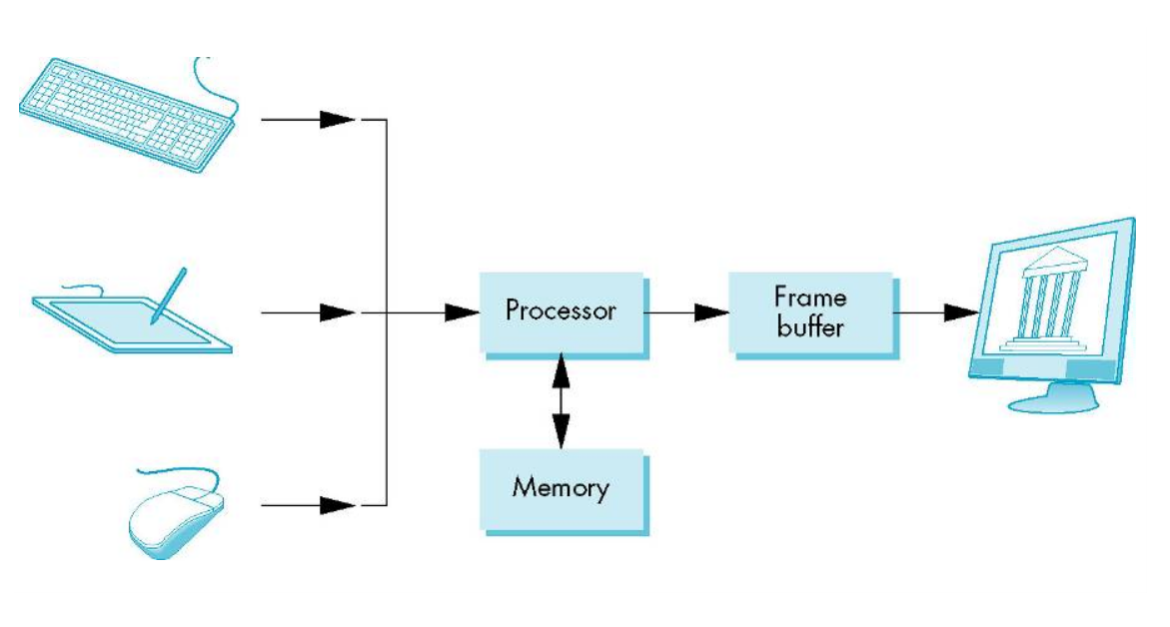
\includegraphics[width=0.8\textwidth]{Figures/framebuffer}
			\caption{\textit{Rasterização}}
		\end{center}
	\end{figure}


\end{frame}

%%%%%%%%%%%%%%%%%%%%%%%%%%%%%%%%%%%%%%%%%%%%%%%%%%%%%%%%%%%%%%%%%%%%%%%%%%%%%%%%%%%%%%%%%%

\begin{frame}
\frametitle{Dispositivo de Exibição Matricial}

	\begin{block}{\textit{Frame Buffer}}
		\begin{itemize}
			\item<1-> A resolução é o número de pixels.
			\item<2-> Implementado com VRAM/DRAM
				\begin{itemize}
					\item Video Randon-acess Memory.
					\item Dynamic Randon-acess Memory.
					\item Acesso rápido para a re-exibição da imagem.
				\end{itemize}
			\item<3-> O \textit{Frame Buffer} armazena também outras informações:
				\begin{itemize}
					\item Informações de camadas.
					\item Informações sobre múltiplos buffers.
				\end{itemize}
			\item<4-> Sistema RGB: Red, Green e Blue.
				\begin{itemize}
					\item A profundidade do \textit{Frame Buffer} define a quantidade de cores possíveis.
					\item 1 bit = 2 cores; 2 bits = $2^2$ = 4 cores; 8 bits = $2^8$ = 256 cores.
				\end{itemize}
			\item<5-> O sistema em geral possui vários processadores gráficos dedicados com funções variadas.

		\end{itemize}
	\end{block}


\end{frame}

%%%%%%%%%%%%%%%%%%%%%%%%%%%%%%%%%%%%%%%%%%%%%%%%%%%%%%%%%%%%%%%%%%%%%%%%%%%%%%%%%%%%%%%%%%

\begin{frame}
\frametitle{Dispositivo de Exibição Matricial}

	\begin{figure}[!h]
		\begin{center}
			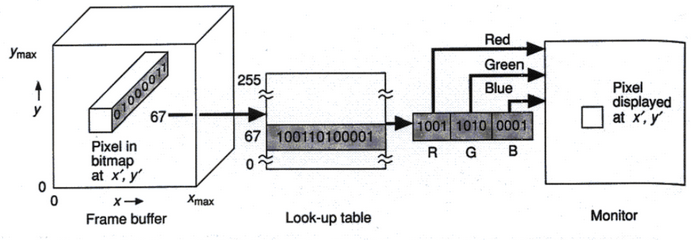
\includegraphics[width=0.8\textwidth]{Figures/lookuptable}
			\caption{\textit{Look-up Table }}
		\end{center}
	\end{figure}
	
	\begin{block}{\textit{Frame Buffer - Look-up Table}}
		\begin{itemize}
			\item Paleta de cores.
			\item Neste exemplo contém uma paleta contém 256 cores das 4096 possíveis.
		\end{itemize}
	\end{block}


\end{frame}


%%%%%%%%%%%%%%%%%%%%%%%%%%%%%%%%%%%%%%%%%%%%%%%%%%%%%%%%%%%%%%%%%%%%%%%%%%%%%%%%%%%%%%%%%%

\begin{frame}
\frametitle{Dispositivo de Exibição Matricial}

	\begin{block}{Placa Gráfica}
		\begin{itemize}
			\item Recebe os comandos para serem desenhados do processador e desenha no vídeo.
			\begin{itemize}
				\item \textit{Drawing} (\textit{Front end}): Recebe do processador as informações de quais pixels serão desenhados e com quais valores. Os pixels são traçados no bitmap (\textit{Frame Buffer}).
				\item Video (\textit{back end}): Interpreta os valores do bitmap, mapeando seus valores para serem exibidos no vídeo.
			\end{itemize}
		\end{itemize}
	\end{block}


\end{frame}


%%%%%%%%%%%%%%%%%%%%%%%%%%%%%%%%%%%%%%%%%%%%%%%%%%%%%%%%%%%%%%%%%%%%%%%%%%%%%%%%%%%%%%%%%%

\begin{frame}
\frametitle{Dispositivo de Exibição Matricial}

	\begin{figure}[!h]
		\begin{center}
			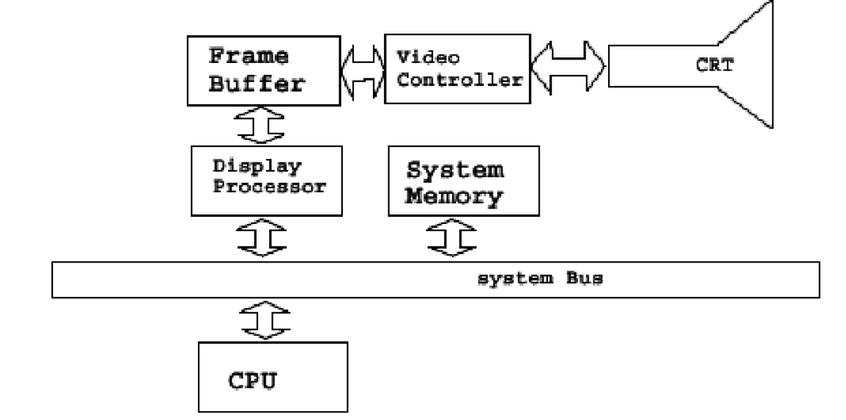
\includegraphics[width=0.9\textwidth]{Figures/arqMatrix}
			\caption{Arquitetura da Exibição Matricial.}
		\end{center}
	\end{figure}
	
\end{frame}

%%%%%%%%%%%%%%%%%%%%%%%%%%%%%%%%%%%%%%%%%%%%%%%%%%%%%%%%%%%%%%%%%%%%%%%%%%%%%%%%%%%%%%%%%%

\begin{frame}
\frametitle{Dispositivo de Exibição Matricial}

	\begin{block}{Vantagens}
		\begin{itemize}
			\item Adequado para imagens coloridas.
			\item Capacidade de integrar imagens digitalizadas e sintetizadas.
			\item Baixo custo.
			\item Rasteio fixo (Tempo de restauração independente da complexidade da cena).
			\item Permite preenchimento de interior de objetos com cores e padrões.
			\item Permite operações com blocos de pixels.
		\end{itemize}
	
	\end{block}
	
\end{frame}

%%%%%%%%%%%%%%%%%%%%%%%%%%%%%%%%%%%%%%%%%%%%%%%%%%%%%%%%%%%%%%%%%%%%%%%%%%%%%%%%%%%%%%%%%%

\begin{frame}
\frametitle{Dispositivo de Exibição Matricial}

	\begin{block}{Desvantagens}
		\begin{itemize}
			\item Requer conversão de imagens digitais para forma matricial.
			\item As transformações não são feitas apenas transformando os extremos do objetos.
			\item Requer muita memória de capacidade de processamento.
			\item Aliasing.
		\end{itemize}
	
	\end{block}
	
\end{frame}


%%%%%%%%%%%%%%%%%%%%%%%%%%%%%%%%%%%%%%%%%%%%%%%%%%%%%%%%%%%%%%%%%%%%%%%%%%%%%%%%%%%%%%%%%%

\begin{frame}
\frametitle{Dispositivo de Exibição Matricial}

	\begin{figure}[!h]
		\begin{center}
			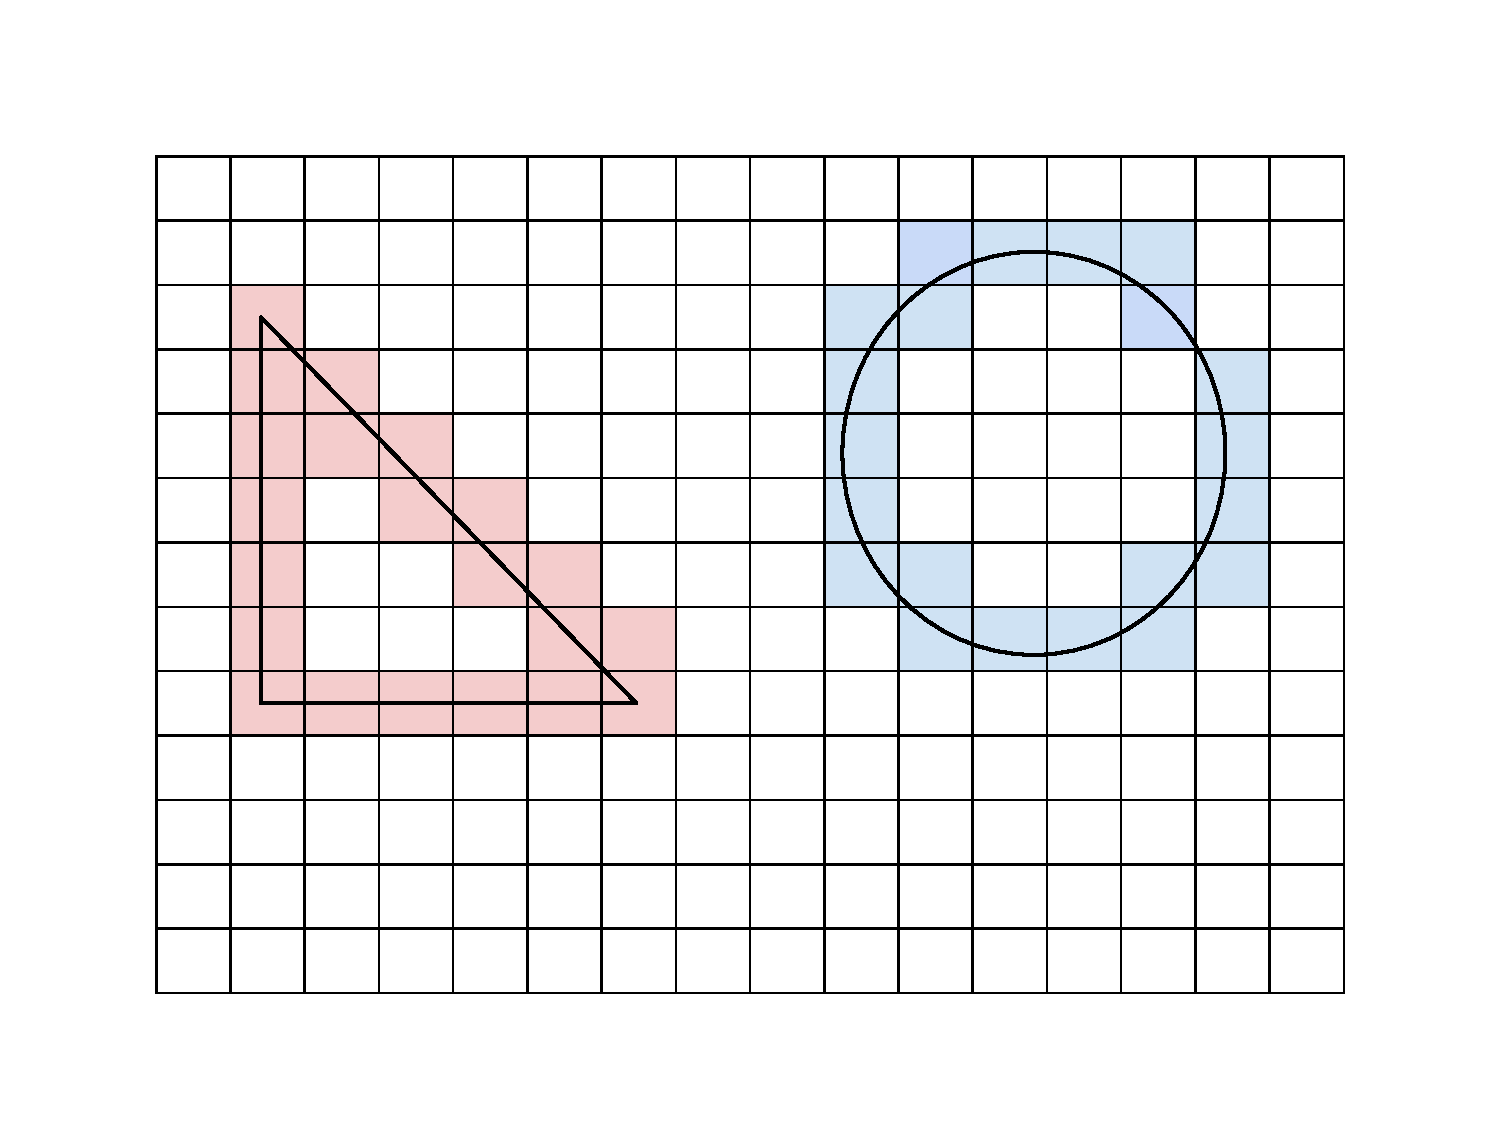
\includegraphics[width=0.8\textwidth]{Figures/aliasing}
			\caption{Exemplo de Aliasing.}
		\end{center}
	\end{figure}
	
\end{frame}

%%%%%%%%%%%%%%%%%%%%%%%%%%%%%%%%%%%%%%%%%%%%%%%%%%%%%%%%%%%%%%%%%%%%%%%%%%%%%%%%%%%%%%%%%%
\subsubsection{Outros Tipos de Tecnologia de Exibição}
\begin{frame}
\frametitle{Outros Tipos de Tecnologia de Exibição}

	\begin{block}{Outras Tecnologias de Exibição de Imagens}
		\begin{itemize}
			\item Possui volume e peso menores.
			\item Possibilita escrever na superfície.
			\begin{itemize}
				\item Emissivos: Convertem energia elétrica em luz (Plasma).
				\item Não Emissivos: Usam efeitos óticos para converter a luz natural em padrões gráficos (LCD, LED).
			\end{itemize}
		\end{itemize}
	\end{block}
	
\end{frame}


%%%%%%%%%%%%%%%%%%%%%%%%%%%%%%%%%%%%%%%%%%%%%%%%%%%%%%%%%%%%%%%%%%%%%%%%%%%%%%%%%%%%%%%%%%
\section{Áreas Relacionadas}
%%%%%%%%%%%%%%%%%%%%%%%%%%%%%%%%%%%%%%%%%%%%%%%%%%%%%%%%%%%%%%%%%%%%%%%%%%%%%%%%%%%%%%%%%%


\begin{frame}
\frametitle{Áreas Relacionadas a Computação Gráfica}

\begin{block}{Áreas Relacionadas a Computação Gráfica}

		\begin{itemize}
			\item Computação Gráfica.
			\item Visão Computacional.
			
		\end{itemize}
\end{block}

\end{frame}



%%%%%%%%%%%%%%%%%%%%%%%%%%%%%%%%%%%%%%%%%%%%%%%%%%%%%%%%%%%%%%%%%%%%%%%%%%%%%%%%%%%%%%%%%%

\subsection{Computação Gráfica}
\begin{frame}
\frametitle{Computação Gráfica}

	\begin{figure}[!h]
		\begin{center}
			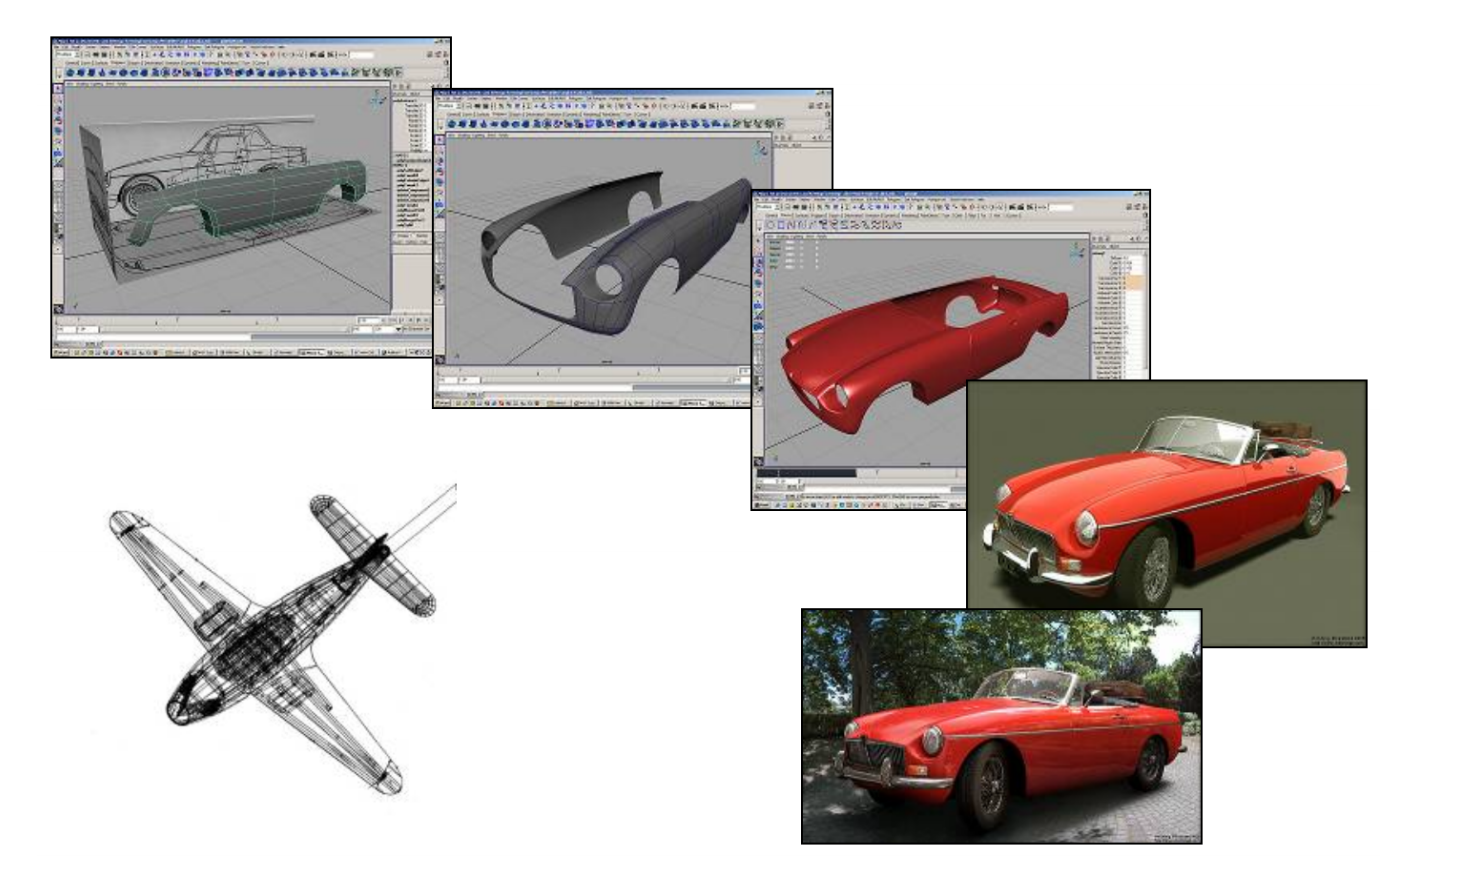
\includegraphics[width=0.8\textwidth]{Figures/cad}
			\caption{Software CAD's.}
		\end{center}
		
	\end{figure}

\end{frame}

%%%%%%%%%%%%%%%%%%%%%%%%%%%%%%%%%%%%%%%%%%%%%%%%%%%%%%%%%%%%%%%%%%%%%%%%%%%%%%%%%%%%%%%%%%


\begin{frame}
\frametitle{Computação Gráfica}

	\begin{figure}[!h]
		\begin{center}
			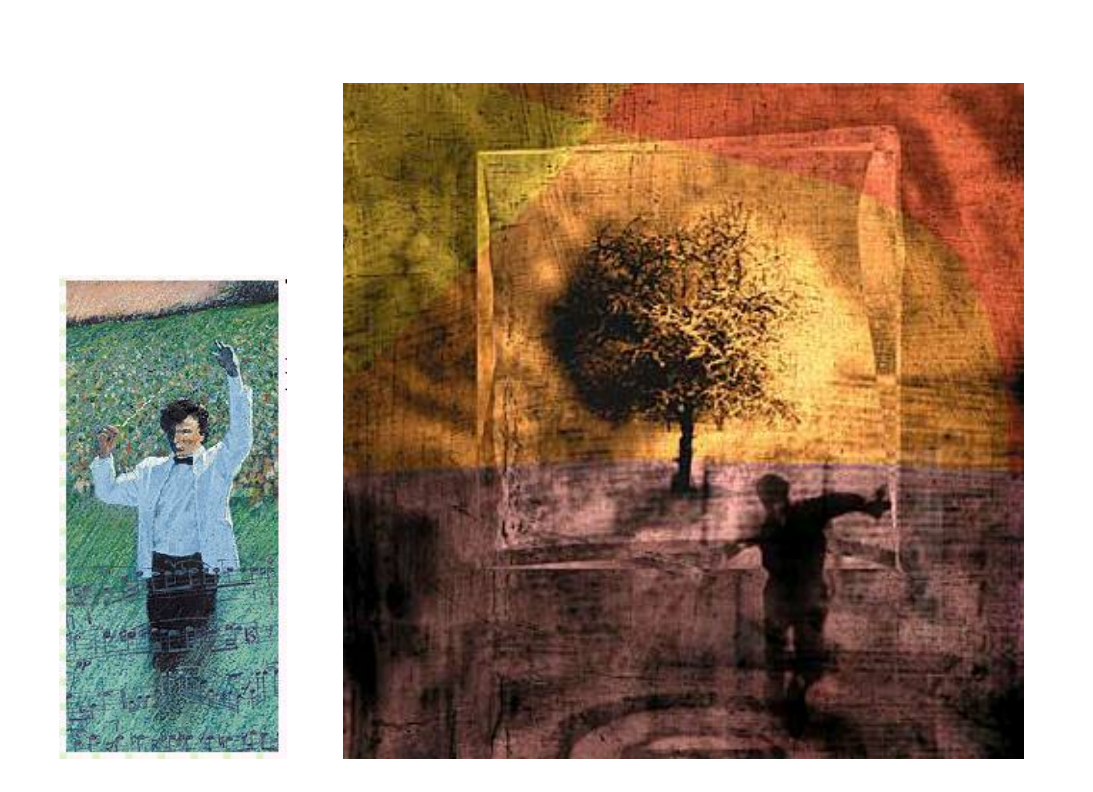
\includegraphics[width=0.8\textwidth]{Figures/arte}
			\caption{Obra de arte feita com Computação Gráfica.}
		\end{center}
		
	\end{figure}

\end{frame}

%%%%%%%%%%%%%%%%%%%%%%%%%%%%%%%%%%%%%%%%%%%%%%%%%%%%%%%%%%%%%%%%%%%%%%%%%%%%%%%%%%%%%%%%%%
\begin{frame}
\frametitle{Computação Gráfica}
	
	\begin{figure}[!h]
		\begin{center}
			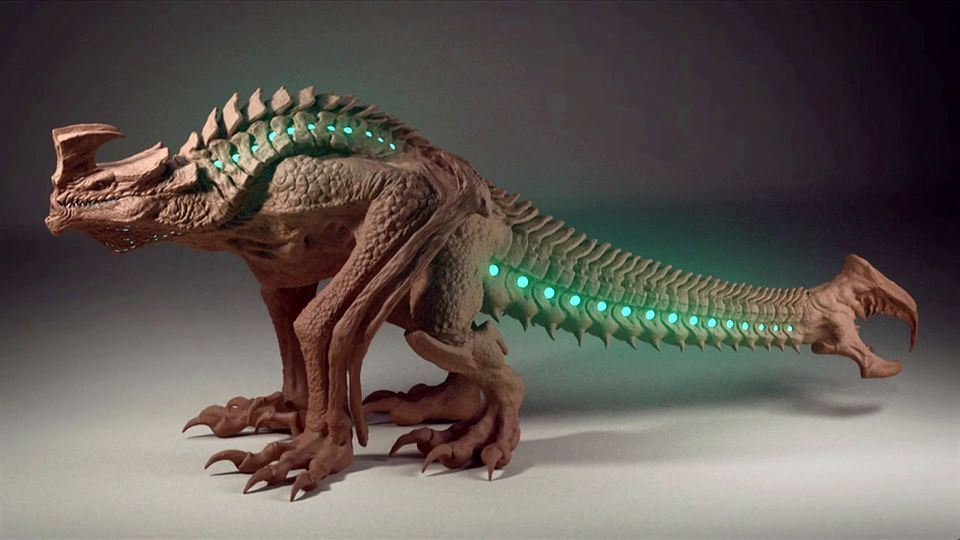
\includegraphics[width=0.9\textwidth]{Figures/pr1}
			\caption{Filme Pacific Rim.}
		\end{center}
		
	\end{figure}
	

\end{frame}



%%%%%%%%%%%%%%%%%%%%%%%%%%%%%%%%%%%%%%%%%%%%%%%%%%%%%%%%%%%%%%%%%%%%%%%%%%%%%%%%%%%%%%%%%%


\begin{frame}
\frametitle{Computação Gráfica}
	
	\begin{figure}[!h]
		\begin{center}
			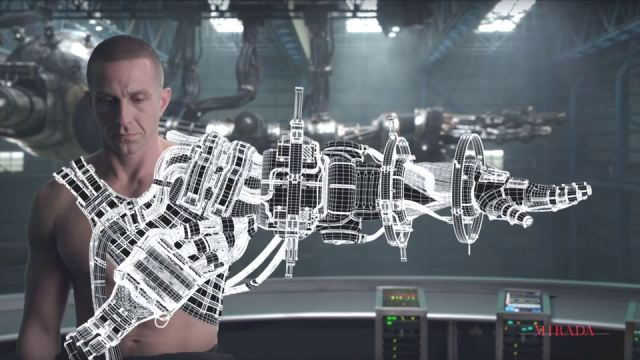
\includegraphics[width=0.9\textwidth]{Figures/pr2}
			\caption{Filme Pacific Rim.}
		\end{center}
		
	\end{figure}
	

\end{frame}


%%%%%%%%%%%%%%%%%%%%%%%%%%%%%%%%%%%%%%%%%%%%%%%%%%%%%%%%%%%%%%%%%%%%%%%%%%%%%%%%%%%%%%%%%%


\begin{frame}
\frametitle{Computação Gráfica}
	
	\begin{figure}[!h]
		\begin{center}
			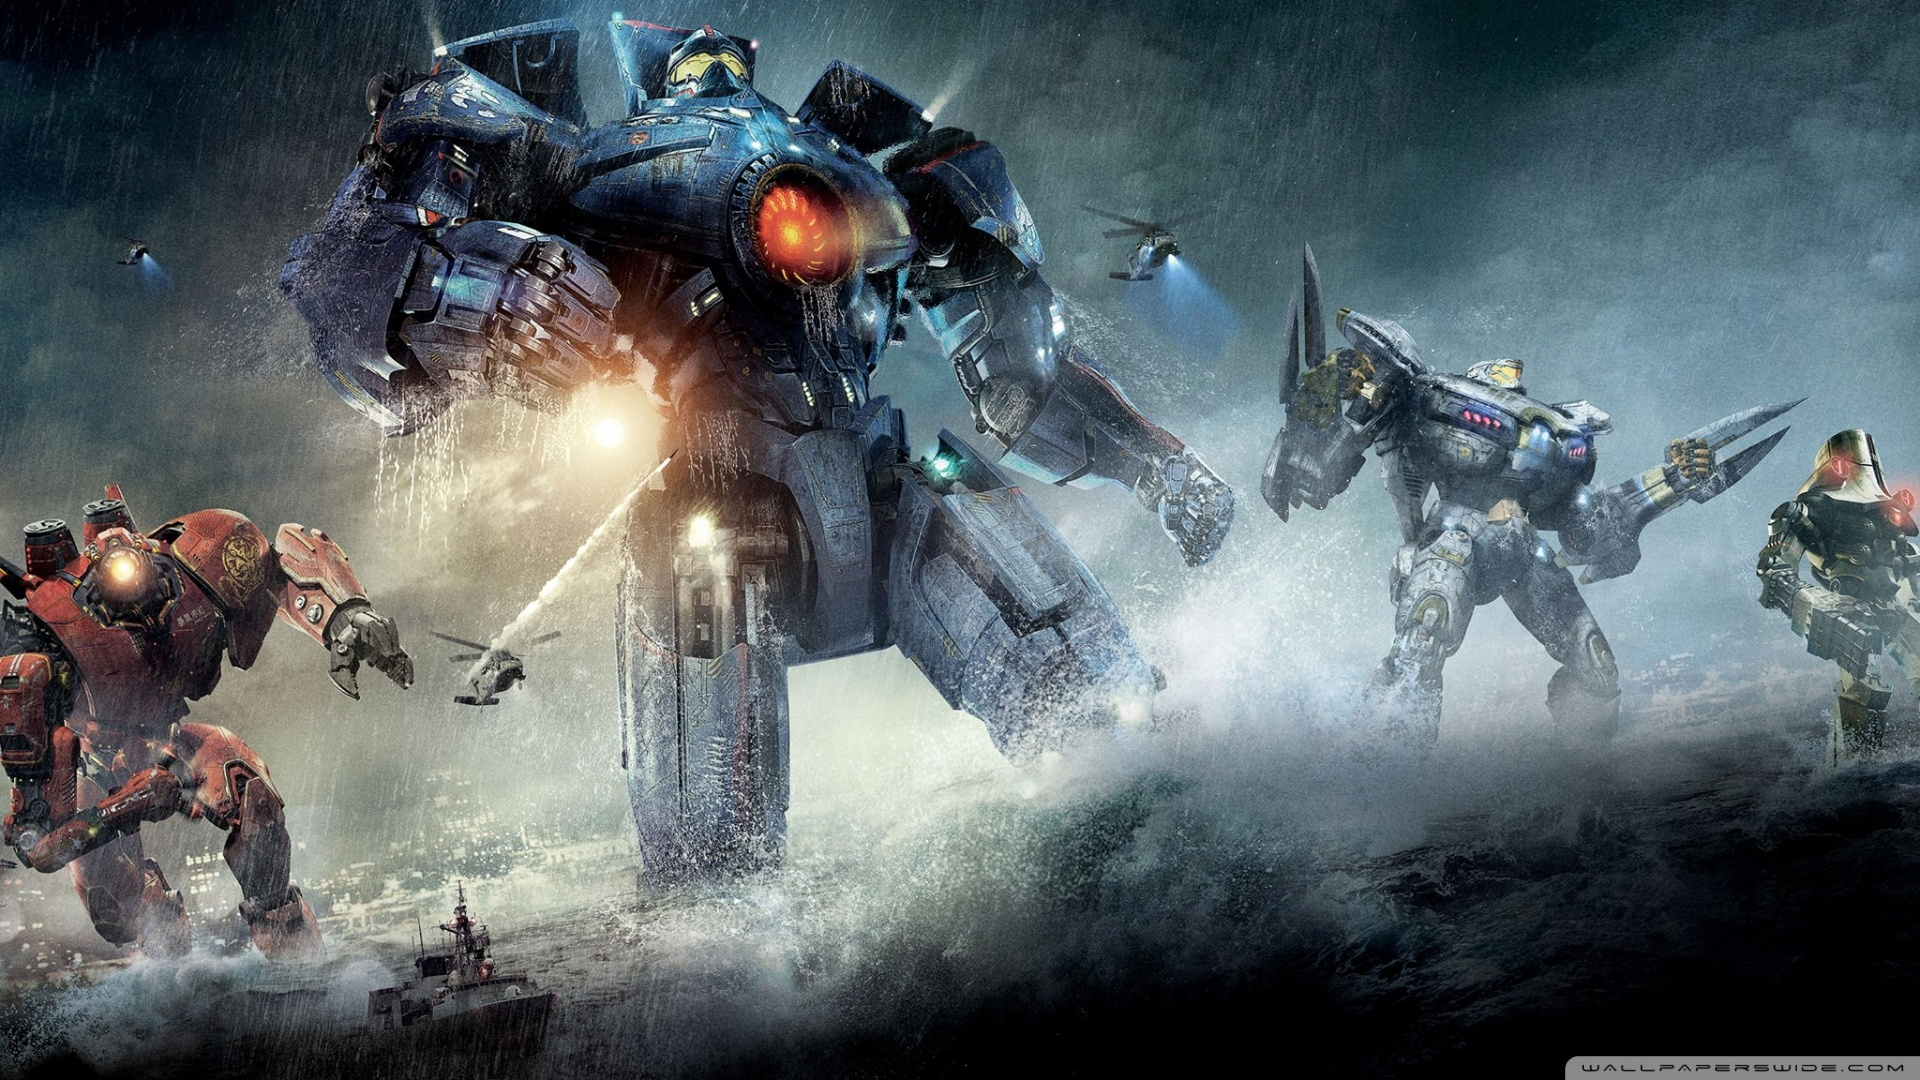
\includegraphics[width=0.9\textwidth]{Figures/pr3}
			\caption{Filme Pacific Rim.}
		\end{center}
		
	\end{figure}
	

\end{frame}


%%%%%%%%%%%%%%%%%%%%%%%%%%%%%%%%%%%%%%%%%%%%%%%%%%%%%%%%%%%%%%%%%%%%%%%%%%%%%%%%%%%%%%%%%%

\subsection{Processamento de Imagens}
\begin{frame}
\frametitle{Processamento de Imagens}

\begin{block}

		\begin{itemize}
			\item<1-> Técnicas de processamento e transformações de imagens em forma de ``matrizes'' pixels.
		\end{itemize}
\end{block}

\begin{block}

		\begin{itemize}
			\item Melhorar características visuais (aumentar contraste, melhorar foco, reduzir ruído, etc..).
			\item Melhorar regiões de interesse e até mesmo ``transformar'' as imagens, criando efeitos visuais.
		\end{itemize}
\end{block}

\end{frame}



%%%%%%%%%%%%%%%%%%%%%%%%%%%%%%%%%%%%%%%%%%%%%%%%%%%%%%%%%%%%%%%%%%%%%%%%%%%%%%%%%%%%%%%%%%


\begin{frame}
\frametitle{Processamento de Imagens}
	
	\begin{figure}[!h]
		\begin{center}
			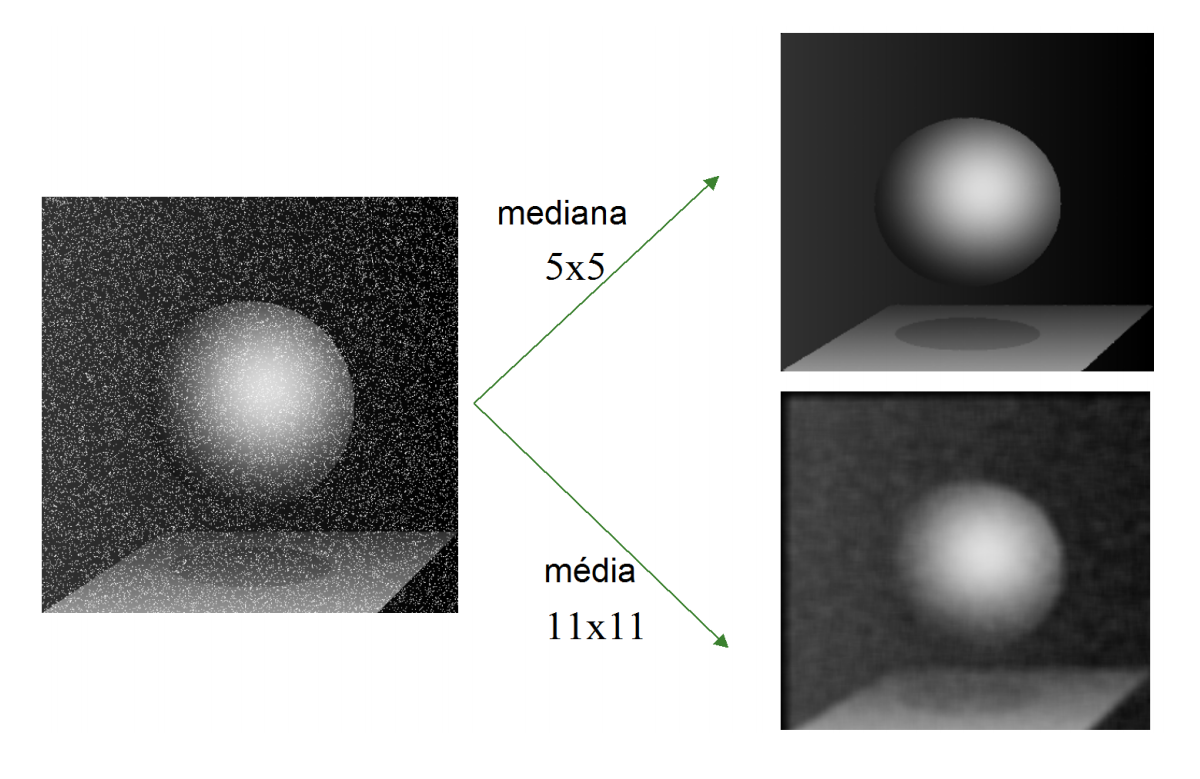
\includegraphics[width=0.9\textwidth]{Figures/pi}
			\caption{Transformações em imagens.}
		\end{center}
		
	\end{figure}
	

\end{frame}

%%%%%%%%%%%%%%%%%%%%%%%%%%%%%%%%%%%%%%%%%%%%%%%%%%%%%%%%%%%%%%%%%%%%%%%%%%%%%%%%%%%%%%%%%%


\begin{frame}
\frametitle{Processamento de Imagens}
	
	\begin{figure}[!h]
		\begin{center}
			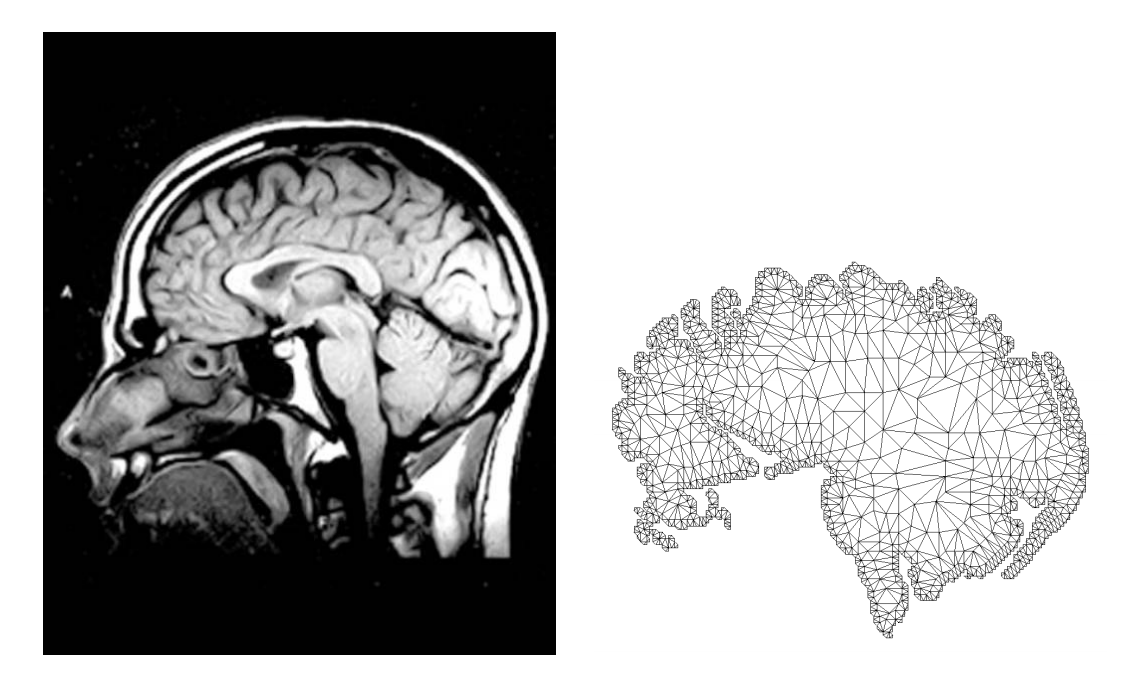
\includegraphics[width=0.9\textwidth]{Figures/cerebro}
			\caption{Representação de um cérebro a partir de uma radiografia.}
		\end{center}
		
	\end{figure}
	
\end{frame}





%%%%%%%%%%%%%%%%%%%%%%%%%%%%%%%%%%%%%%%%%%%%%%%%%%%%%%%%%%%%%%%%%%%%%%%%%%%%%%%%%%%%%%%%%%

\begin{frame}
\frametitle{Referências}
		\begin{block}{Bibliografia Básica}
			
			\begin{itemize}
				\item FOLEY, J. D. et alii. Introduction to Computer Graphics. Reading: Addison Wesley, 1994.*
				\item FOLEY, J. D. et. alii. Computer Graphics: Principles and Practice. Reading: Addison Wesley, 1990. 
			\end{itemize}

		\end{block}
		
		\begin{block}{Bibliografia Básica}
			
			\begin{itemize}
				\item TORI, Romero; FILGUEIRAS, Lucia Vilela Leila; ARAKAKI, Reginaldo; MASSOLA, Antonio Marcos Aguirra. Fundamentos de computação gráfica: compugrafia. Rio de Janeiro: LTC, 1987. 356 p. ISBN 85-216-0506-4.
				
				\item GOMES, J. et. alii. Fundamentos da Computação Gráfica. IMPA: Série de Computação e Matemática, 2008.
				
				\item KLAWONN, Frank. Introduction to Computer Graphics: Using Java 2D and 3D. Springer London, 2008. 
			\end{itemize}

		\end{block}

	\begin{figure}[!h]
		\begin{center}
			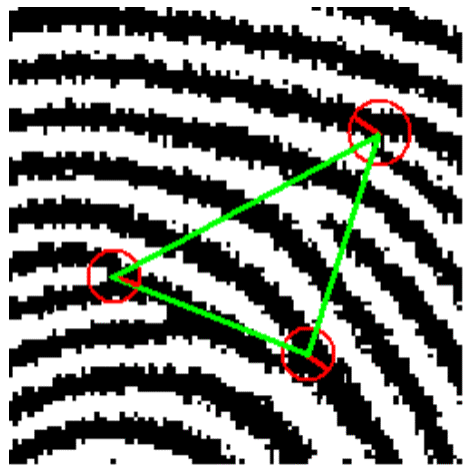
\includegraphics[width=0.5\textwidth]{Figures/semelhancas}
		\end{center}
		
	\end{figure}
	
\end{frame}


%%%%%%%%%%%%%%%%%%%%%%%%%%%%%%%%%%%%%%%%%%%%%%%%%%%%%%%%%%%%%%%%%%%%%%%%%%%%%%%%%%%%%%%%%%
\begin{frame}

	\begin{block}{Referência}
		Esta apresentação foi baseada na apresentação do porf. Fernando V. Paulovitch (USP - ICMC).
	\end{block}
	
\end{frame}

%----------------------------------------------------------------------------------------

\end{document} 